%%%%%%%%%%%%%%%%%%%%%%%%%%%%%%
%%%%%%%%%%%%%%%%%%%%%%%%%%%%%%
SLIDE senza testata senza titolone
%%%%%%%%%%%%%%%%%%%%%%%%%%%%%%

\thispagestyle{empty}
\begin{frame}
   \vspace{-1.5cm}
   zzz
\end{frame}

%%%%%%%%%%%%%%%%%%%%%%%%%%%%%%
%%%%%%%%%%%%%%%%%%%%%%%%%%%%%%
SLIDE senza testata con titolone
%%%%%%%%%%%%%%%%%%%%%%%%%%%%%%

\thispagestyle{empty}
\begin{frame}
   \vspace{-1.5cm}
   \frametitle{Titolone}
   zzz
\end{frame}

%%%%%%%%%%%%%%%%%%%%%%%%%%%%%%
%%%%%%%%%%%%%%%%%%%%%%%%%%%%%%
SLIDE con testata titoletto senza titolone
%%%%%%%%%%%%%%%%%%%%%%%%%%%%%%
\subsection{TITOLETTO}
\begin{frame}
   zzz
\end{frame}

%%%%%%%%%%%%%%%%%%%%%%%%%%%%%%
%%%%%%%%%%%%%%%%%%%%%%%%%%%%%%
SLIDE con testata titoletto e con titolone
%%%%%%%%%%%%%%%%%%%%%%%%%%%%%%
\subsection{ALGEBRA DEI VETTORI CIRCOLANTI CONCATENATI}
\begin{frame}
  \frametitle{Titolone}
  zzz
\end{frame}

%%%%%%%%%%%%%%%%%%%%%%%%%%%%%%
%%%%%%%%%%%%%%%%%%%%%%%%%%%%%%
SLIDE con diagramma
%%%%%%%%%%%%%%%%%%%%%%%%%%%%%%

\begin{frame}
   \begin{center}
   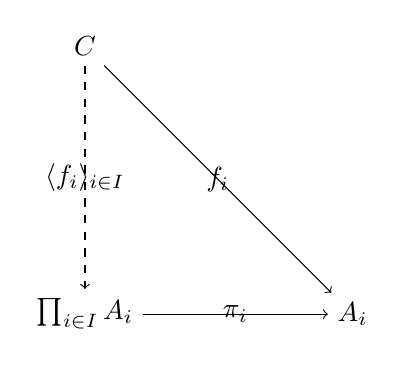
\begin{tikzpicture}
    \node (C) {$C$};
    \node (P) [node distance=3.4cm, below of=C] {$\prod_{i \in I} A_i$};
    \node (Ai) [node distance=3.4cm, right of=P] {$A_i$};
    \draw[->] (C) to node {$f_i$} (Ai);
    \draw[->, dashed] (C) to node [swap] {$\langle f_i \rangle_{i \in I}$} (P);
    \draw[->] (P) to node [swap] {$\pi_i$} (Ai);
   \end{tikzpicture} 
   \end{center}
\end{frame}

%%%%%%%%%%%%%%%%%%%%%%%%%%%%%%
%%%%%%%%%%%%%%%%%%%%%%%%%%%%%%
%%%%%%%%%%%%%%%%%%%%%%%%%%%%%%
%%%%%%%%%%%%%%%%%%%%%%%%%%%%%%
%%%%%%%%%%%%%%%%%%%%%%%%%%%%%%
%%%%%%%%%%%%%%%%%%%%%%%%%%%%%%
%% DIAGRAMMI:
%%%%%%%%%%%%%%%%%%%%%%%%%%%%%%
%%%%%%%%%%%%%%%%%%%%%%%%%%%%%%


 \begin{tikzpicture}[xscale=1.5,yscale=3]

\path node   (m11) at (0,0) {$N_1$}         (-1,0) node[anchor=east] {$e_1$ \ :}       
      node   (m12) at (3,0) {$G_1$}         
      node   (m13) at (5,0) {$Q_1$}
      node   (m21) at (0,1) {$N_1\times A$} (-1,1) node[anchor=east] {$e_1\times A$ \ :}  
      node   (m22) at (3,1) {$G_1\times A$} 
      node   (m23) at (5,1) {$Q_1$} 
      node   (m31) at (0,2) {$\displaystyle\frac{ N_1\times A}{\alpha A}$} 
                      (-1,2)  node[anchor=east]{$nat'(e_1\times A)=
                                 \displaystyle\frac{ e_1\times A}{\alpha N_1}$ \ :}        
      node   (m32) at (3,2) {$\displaystyle\frac{ G_1\times A}{\beta\lambda N_1}$} 
      node   (m33) at (5,2) {$Q_1$} 
      node   (m41) at (0,3) {$N_1\times A$} (-1,3) node[anchor=east] {$e_1\times A$ \ :}           
      node   (m42) at (3,3) {$G_1\times A$} 
      node   (m43) at (5,3) {$Q_1$} 
      node   (m51) at (0,4) {$N_1\times N_2$} (-1,4) node[anchor=east] {$\tilde{e}$ \ :} 
      node   (m52) at (3,4) {$\tilde{G}$} 
      node   (m53) at (5,4) {$Q$} 
      node   (m61) at (0,5) {$N_2$} (-1,5) node[anchor=east] {$e_2$ \ :}           
      node   (m62) at (3,5) {$G_2$}         
      node   (m63) at (5,5) {$Q_2$} ;
     { [ thick]
      \draw[>->]   (m61) -- node[above]{$\kappa_2$}      (m62); 
      \draw[->>]   (m62) -- node[above]{$\pi_2$}    (m63);
      \draw[>->]   (m51) -- node[above]{$\lambda$}  (m52);  
      \draw[>->>]  (m52) -- node[above]{$\beta$}    (m53);    
      \draw[->>]   (m42) -- (m43);  
      \draw[>->]   (m31) -- (m32); 
      \draw[->>]   (m32) -- (m33);
      \draw[->>]   (m22) -- (m23);
      \draw[>->]   (m11) -- node[above]{$\kappa_1$}      (m12); 
      \draw[->>]   (m12) -- node[above]{$n_1$}      (m13);

      {[>->,shorten >=.5cm]
      \draw        (m41) -- (m42); 
      \draw        (m21) -- (m22); 
      }

      {[->>]       
      \draw   (m51) -- node[right]{$\sigma_2$} (m61); 
      \draw   (m52) -- node[right]{$\tau_2$}   (m62);
      \draw   (m21) -- node[right]{nat'}       (m31); 
      \draw   (m22) -- node[right]{nat}        (m32);  
      \draw   (m41) -- node[right]{nat'}       (m31); 
      \draw   (m42) -- node[right]{nat}        (m32);
      }
      \draw[->]    (m11) -- node[right]{$\mu'$}     (m21);  
      \draw[->]    (m12) -- node[right]{$\mu$}      (m22);  
      \draw[>->>]  (m53) -- node[right]{$\gamma_2$} (m63);  
      \draw[>->>]  (m53) -- node[right]{$\gamma_1$} (m43); 
      \draw[>->]   (m51) -- node[right]{$\alpha$}   (m41); 
      \draw[>->]   (m52) -- node[right]{$\beta$}    (m42);  
      {[dashed] 
       {[->]
       \draw   (m51) to [out=-140,in= 140]      (m31);
       \draw   (m52) to [out=-140,in= 140]      (m32);
       }
       {[>->]
       \draw  (m11) to [out= 140,in=-140]      (m31); 
       \draw  (m12) to [out= 140,in=-140]      (m32);} 
       }
       \draw[double]  (m43)--(m33)--(m23)--(m13);
       }
\end{tikzpicture}


%%% 
STRATEGIE
Usare \pause solo per le slide empty. In generale scrivere meno frasi possibili, usare di più i simboli.
i diagrammi e gli esempi sono da mettere sempre nelle slide empty.



   \begin{center}
   \begin{tikzpicture}[xscale=1.5,yscale=1.5]

\path node   (V) at (0,0) {$\mathcal{V}_{r, \mathbb{F}}^{c}$}         %(-1,0) node[anchor=east] {$e_1$ \ :}       
      node   (M) at (4,0) {$ \mathcal{M}_{r,\mathbb{F} }^{c} $}         
      node   (R) at (0,3) {$ \quotient{ \mathbb{F}[x] }{ (x^r -1 )}$} %(-0.9,3) node[anchor=east] {$\mathcal{R}_{r, \mathbb{F}}$ \ =}
      node   (A) at (4,3) {$\mathbb{F}C_{r}$} %(-1,1) node[anchor=east] {$e_1\times A$ \ :}  
      ;
     { %[ thick]
      \draw[->]   (R) -- node[above]{$\psi_4$}     (A); 
      \draw[->]   (V) -- node[above]{$\psi_1$}     (M);
      \draw[->]   (R) -- node[right]{$\psi_2$}     (V);  
      \draw[->]   (A) -- node[right]{$\psi_3$}     (M);     
      }
\end{tikzpicture}
   \end{center}

\[
\begindc{\commdiag}[3]
%insiemi
\obj(0,12)[A]{$ \lbrace A \mid A \subseteq \mathscr{L} \rbrace $}
%[R]{$ \lbrace \mathfrak{a} \mid \mathfrak{a} \trianglelefteq \mathcal{R}_{r,q} \rbrace $}
\obj(50,24)[O]{$ \lbrace \cup_{t \in A} O(t)  \mid A \subseteq \mathscr{L} \rbrace $}
%[A]{$ \lbrace A \mid A \subseteq \mathscr{L} \rbrace $}
\obj(50,0)[R]{$ \lbrace \mathfrak{a} \mid \mathfrak{a} \trianglelefteq \mathcal{R}_{r,q} \rbrace $}
%[O]{$ \lbrace \cup_{t \in A} O(t)  \mid A \subseteq \mathscr{L} \rbrace $}


%frecce
\mor{A}{R}{}
\mor{A}{O}{}
\mor{O}{R}{}

\enddc
\]



Sia $\mathbb{F} = \mathbb{Q}$ ed $r = 7$ allora
\begin{align*}
  x^{7} - 1 &= \Phi_{1}(x) \Phi_{7}(x) \\
            &= (x-1)(x^6 +x^5 + x^4 + x^3 +x^2 + x +1)
\end{align*}
Sia $\xi_{7}$ radice primitiva settima:\\
$\xi_{7}^{0} = 1$ è radice di $x-1$.\\
$\xi_{7}^{j}$ è radice di $\Phi_{7}(x)$ per $j = 1, \dots ,6 $.\\
Come prima gli esponenti delle radici primitive settime che soddisfano lo
stesso polinomio ciclotomico sono raggruppate nelle orbite dell'azione di
$\mathbb{Z}_{7}^{\star}$ su $\mathbb{Z}_{7}$: \\
$O(0)= \lbrace 0 \rbrace$.\\
$O(1)= \lbrace 1,2,3,4,5,6 \rbrace$.\\
Mentre se fattorizziamo $ x^{7} - 1$ sul campo $\mathbb{F} = \mathbb{Z}_{2}$,
otteniamo il prodotto
\begin{align*}
  x^{7} - 1 &= M^{(0)}(x) M^{(1)}(x) M^{(3)}(x) \\
            &= (x-1)(x^3 + x + 1)(x^3 + x^2 + 1) 
\end{align*}
Le radici primitive settime si distribuiscono nel modo seguente: \\
$\xi_{7}^{0} = 1$ è radice di $M^{(0)}(x) = x-1$.\\
$\xi_{7}^{1}, \xi_{7}^{2}, \xi_{7}^{4}$ sono radici di $M^{(1)}(x) = x^3 + x +
1$.\\
$\xi_{7}^{3}, \xi_{7}^{5}, \xi_{6}^{1}$ sono radici di $M^{(3)}(x)= x^3 + x^2 +
1$.\\
$G = \lbrace 1,2,4 \rbrace \triangleleft \mathbb{Z}_{7}^{\star}$ 
$O(0)= \lbrace 0 \rbrace$.\\
$O(1)= \lbrace 1,2,4 \rbrace$.\\
$O(3)= \lbrace 3,5,6 \rbrace$.\\



Quindi $ \mathcal{R}_{7, \mathbb{Q}} $ si scompone nel prodotto di due
campi, 
\begin{align*}
\quotient{\mathbb{Q} \lbrack x \rbrack  }{(x^{7} - 1)}
\cong
\quotient{\mathbb{Q} \lbrack x \rbrack  }{\Phi_{1}(x)}
\times
\quotient{\mathbb{Q} \lbrack x \rbrack  }{\Phi_{7}(x)}
\end{align*}
mentre $\mathcal{R}_{7, \mathbb{Z}_{2}}$ si scompone in tre campi.
\begin{align*}
\quotient{\mathbb{Z}_{2} \lbrack x \rbrack  }{(x^{7} - 1)}
\cong
\quotient{\mathbb{Z}_{2} \lbrack x \rbrack  }{M^{(0)}(x)}
\times
\quotient{\mathbb{Z}_{2} \lbrack x \rbrack  }{M^{(1)}(x)}
\times
\quotient{\mathbb{Z}_{2} \lbrack x \rbrack  }{M^{(3)}(x)}
\end{align*}


    \path node   (Q) at (-4.5,3) {$  \prod_{v\in \mathscr{L}} \mathbb{F}(\xi^{v})$}         
	  node   (P) at (0,6) {$ \prod_{v\in \mathscr{L}} \quotient{\mathbb{F} \lbrack x \rbrack  }{M^{(v)}(x)}$} 
	  node   (R) at (0,3) {$\quotient{\mathbb{F} \lbrack x \rbrack  }{ (x^{r} - 1)} $} 
	  node   (V) at (0,0) {$\mathcal{V}_{r, \mathbb{F}}^{c}$}         %(-1,0) node[anchor=east] {$e_1$ \ :}       
          node   (M) at (4,0) {$ \mathcal{M}_{r,\mathbb{F} }^{c} $}         
          node   (A) at (4,3) {$\mathbb{F}C_{r}$} 

          
          
          
          
 \thispagestyle{empty}
\begin{frame}
   \vspace{-1.5cm}
   \begin{center}
     \begin{tikzpicture}[xscale=0.7,yscale=0.7]

      \path node   (VL) at (3,1.7) {$\mathcal{V}_{r,\mathbb{F}}^{\mathscr{L} }$}  
            node   (P) at (1,-1.7) {$ \prod_{v\in \mathscr{L}} \quotient{\mathbb{F} \lbrack x \rbrack  }{M^{(v)}(x)}$} 
            node   (Q) at (5,-1.7) {$  \prod_{v\in \mathscr{L}} \mathbb{F}(\xi^{v})$}
            %%
            node   (V) at (-3,2) {$\mathcal{V}_{r, \mathbb{F}}^{c}$}  
	    node   (M) at (-1,0) {$ \mathcal{M}_{r,\mathbb{F} }^{c} $}         
	    node   (R) at (-5,0) {$\quotient{\mathbb{F} \lbrack x \rbrack  }{ (x^{r} - 1)} $} 
	    node   (A) at (-3,-2) {$\mathbb{F}C_{r}$} 
	    %%
	    node   (N1) at (0,4) {} 
	    node   (N2) at (0,-4) {} 
	    ;
	  { [ thick]
	    \draw[-]   (N2) --     (N1); 
	    }
	    {
	    \draw[->]   (V) -- node[above]{$\gamma$}     (VL); 
	    }
      \end{tikzpicture}
   \end{center}
\end{frame}